\chapter{Auenland DNS}\label{sec:dns-auenland}
Ein DNS-Server im \textit{Auenland}-Netz mit der IP-Adresse \url{10.0.68.110}.\\

\cvss{av=local, ac=low, pr=none, ui=required, s=changed, c=high, i=low, a=low}
\cvssdescription{Brute-Force-Angriff auf den SSH-Login des DNS-Servers mit bekannten Nutzernamen und einer Passwortliste.}

\section{\makecvssbadge Broken Authentication}
\cvssaddtosummary{Auenland DNS-Server: Broken Authentication}
\subsection*{Proof of concept}
Durch die Kompromittierung des Nextcloud-Servers konnte herausgefunden werden, dass der DNS-Server \textit{Auenland} durch den Benutzer \textit{pippin} administriert wird. Daher wurde ein Brute-Force-Angriff auf das SSH-Login des DNS-Servers durchgeführt. Als Benutzernamen wurden \textit{admin} und \textit{pippin}gewählt und für die Passwörter wurde eine Passwortliste verwendet. Durch diesen Brute-Force-Angriff war es möglich, die gültigen Credentials für den Benutzer \textit{pippin} zu erlangen und sich mit diesem per SSH auf dem DNS-Server zu verbinden. Ein Nachweis ist in \autoref{fig:10_dns_proof} dargestellt.\\

\begin{figure}[!ht]
    \centering
    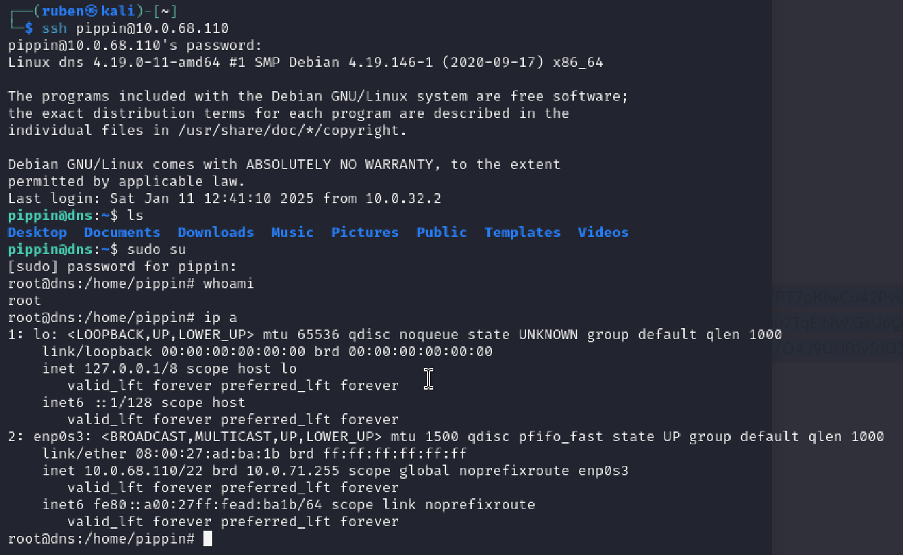
\includegraphics[width=\linewidth]{images/proofs/10_dns_proof.png}
    \caption{Proof für den DNS Server Auenland}
    \label{fig:10_dns_proof}
\end{figure}

\subsection*{Empfehlungen}
\begin{itemize}
    \item Strenge Passwortrichtlinien: Erzwingen Sie die Verwendung komplexer und langer Passwörter und ändern Sie Standardpasswörter, um einfache Passwörter zu vermeiden (siehe \cite{bsi_passwords}).
    \item Account-Sperrung und Ratenbegrenzung: Implementieren Sie Mechanismen, die nach mehreren fehlgeschlagenen Anmeldeversuchen eine Sperrung oder Verzögerung auslösen, um automatisierte Angriffe zu verhindern (siehe \cite{owaspAuthenticationOWASP}).
    \item Multi-Faktor-Authentifizierung (MFA): Ergänzt die Passwortauthentifizierung um einen zusätzlichen Faktor, um den Zugriff auch mit kompromittierten Zugangsdaten zu verhindern (siehe \cite{owaspAuthenticationOWASP}).
\end{itemize}